\chapter{Web Application, Discussion and Conclusion}
\section{Streamlit Web Application}
A Streamlit web application is associated with this project and is available at:
\begin{center}
\url{https://human-activity-recognition-ehccfyncz87dfyderptkah.streamlit.app/}
\end{center}

The notebook includes an export step that prepares files for the application. The exported artifacts include the fitted KNN, Decision Tree and Random Forest models in Joblib format, the test feature and label data in CSV format, a CSV file containing Random Forest feature importance, and a JSON metadata file. The metadata includes the feature names, activity mapping, evaluation results, best-model name and dataset dimensions.

\begin{table}[H]\centering
\caption{Files exported for the web application}
\begin{tabular}{lp{8.2cm}}
\toprule
\textbf{Artifact} & \textbf{Purpose recorded by the notebook}\\
\midrule
\texttt{knn\_har\_model.pkl} & Saved KNN pipeline.\\
\texttt{decision\_tree\_har\_model.pkl} & Saved Decision Tree classifier.\\
\texttt{random\_forest\_har\_model.pkl} & Saved Random Forest classifier.\\
\texttt{X\_test.csv} & Exported test feature matrix.\\
\texttt{y\_test.csv} & Exported test activity labels.\\
\texttt{feature\_importance.csv} & Random Forest feature importance values.\\
\texttt{metadata.json} & Feature names, class mapping, metrics, selected model and dataset dimensions.\\
\bottomrule
\end{tabular}
\end{table}

\subsection{Application Screenshots}
Insert screenshots captured directly from the deployed Streamlit application in the \texttt{screenshots} folder. Suggested screenshots are the application landing page, the activity prediction interface, an example prediction result, and any model-performance or visualisation page that is actually present in the deployed application.

\begin{figure}[H]\centering
\IfFileExists{screenshots/app_home.png}
{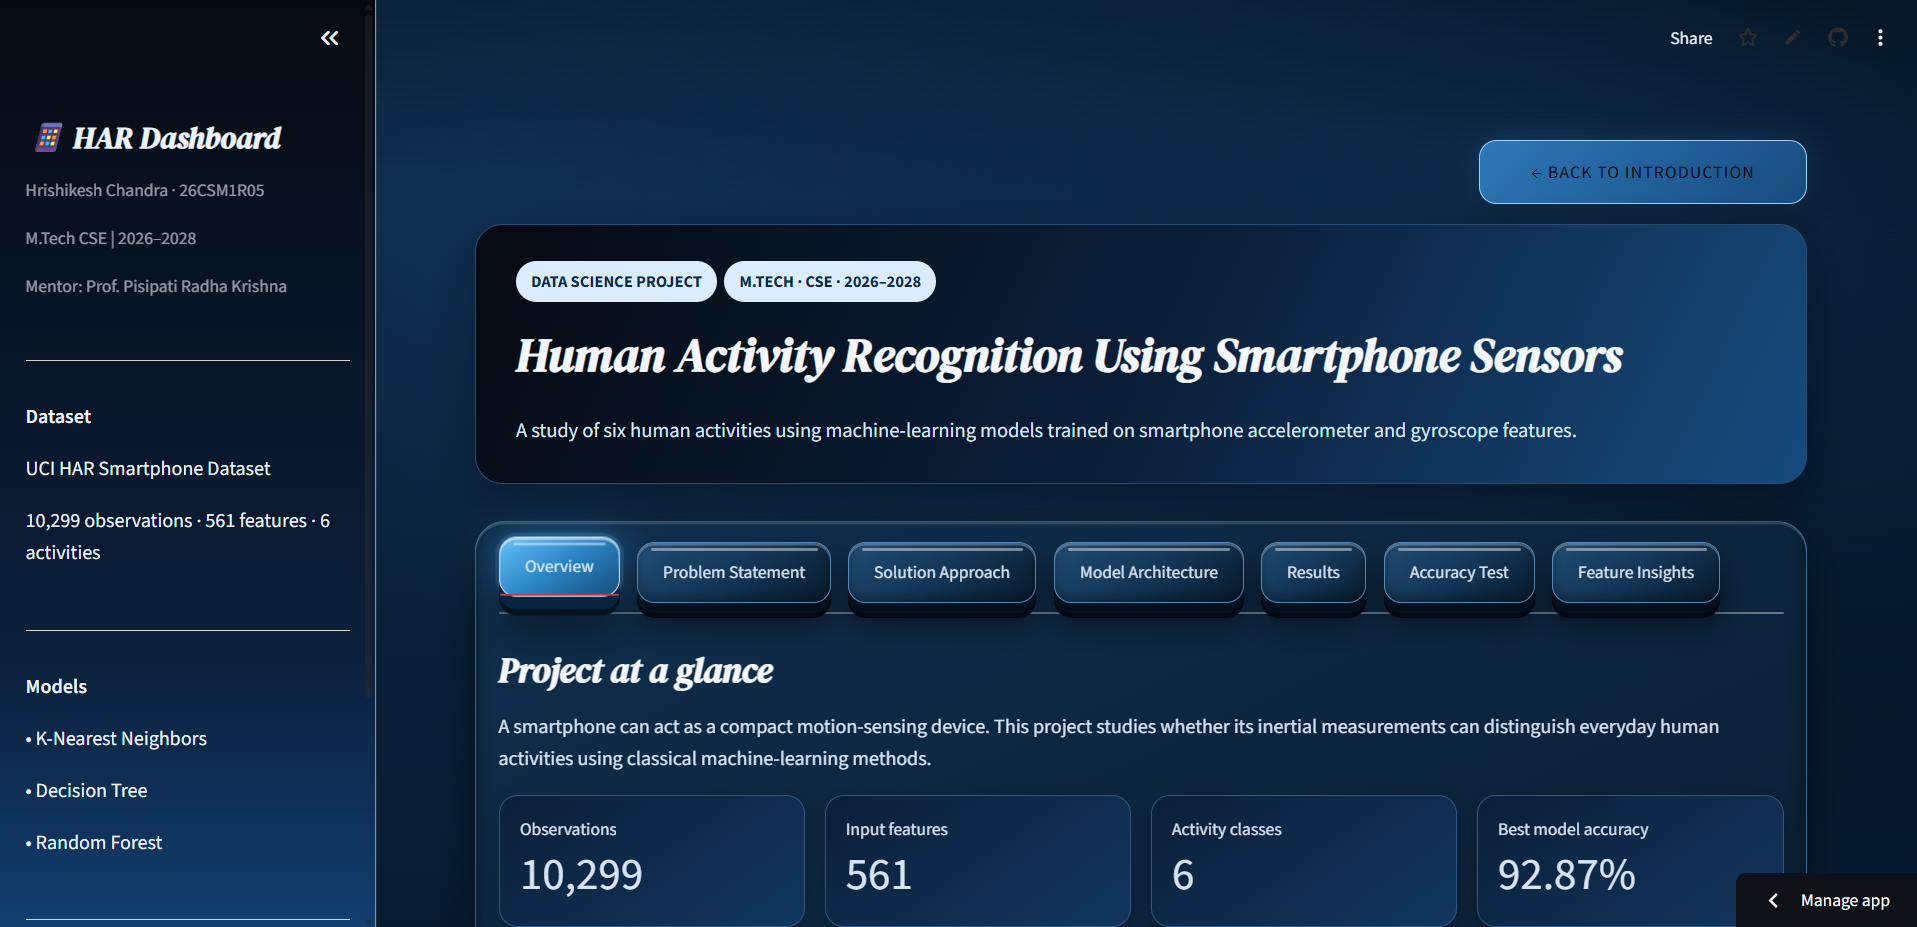
\includegraphics[width=0.92\textwidth]{screenshots/app_home.png}}
{\fbox{\parbox[c][5cm][c]{0.88\textwidth}{\centering Insert screenshot: Streamlit application home page\\[0.2cm]\texttt{screenshots/app\_home.png}}}}
\caption{Streamlit application home page.}
\end{figure}

\begin{figure}[H]\centering
\IfFileExists{screenshots/app_prediction.png}
{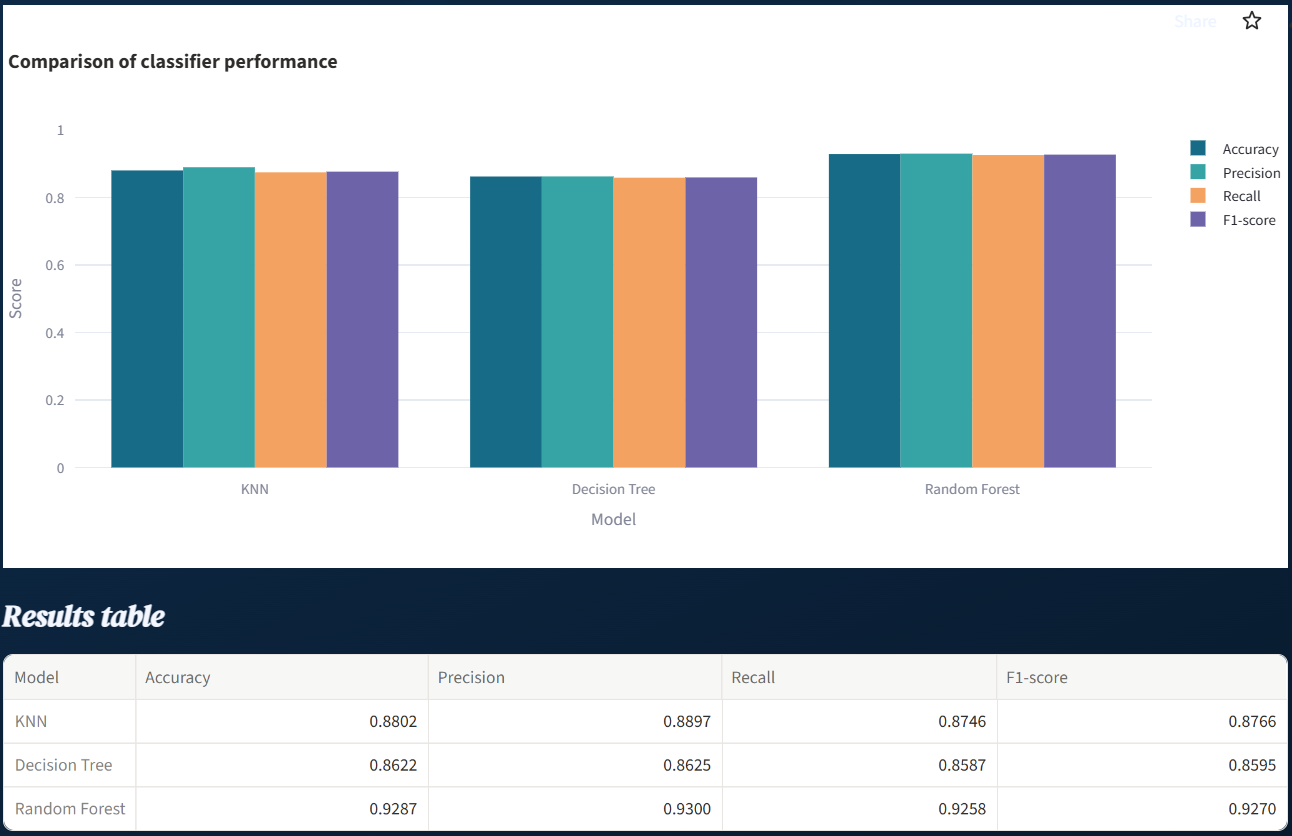
\includegraphics[width=0.92\textwidth]{screenshots/app_prediction.png}}
{\fbox{\parbox[c][5cm][c]{0.88\textwidth}{\centering Insert screenshot: activity prediction result\\[0.2cm]\texttt{screenshots/app\_prediction.png}}}}
\caption{Example activity prediction in the web application.}
\end{figure}

\textit{Note: The application URL was supplied for this report, but its live page could not be retrieved for independent inspection during report preparation. The screenshots and exact user-interface behaviour should therefore be confirmed using the deployed application before final submission.}

\section{Discussion}
The experimental results show that ensemble learning provides the strongest performance among the three models tested on this feature dataset. Random Forest outperforms KNN and Decision Tree on all four reported aggregate metrics. Its macro F1-score of 92.70\% indicates that its performance is strong when the six classes are weighted equally.

The confusion matrices show that laying is identified particularly well by the three classifiers. The most persistent ambiguity for the best model is between sitting and standing, and between walking and walking downstairs. This is reasonable in the context of sensor-based recognition because some activities can produce related movement or posture patterns in the engineered feature space. This interpretation is qualitative; the project does not include a separate causal or sensor-level investigation.

\section{Limitations}
\begin{itemize}
\item The notebook uses a prepared feature dataset rather than acquiring and processing live sensor streams.
\item The project does not demonstrate deployment on a physical wearable device or microcontroller.
\item The reported results are based on the supplied train/test partition; no additional cross-validation or external-dataset evaluation is shown in the notebook.
\item The notebook evaluates three classifiers with the specified configurations. Further hyperparameter optimisation may change the results.
\item The web application is linked in the report, but application screenshots and live behaviour must be verified by the project team before submission.
\item The model predicts only the six activity categories represented in the training labels; it is not designed to identify arbitrary activities outside these classes.
\end{itemize}

\section{Future Enhancements}
Possible future extensions include collecting live accelerometer and gyroscope readings, implementing the documented filtering and feature-extraction pipeline on incoming sensor windows, evaluating the model on data from unseen users, optimising model size and inference latency, and extending the activity label set. The web application can also be enhanced with clearer prediction confidence information and a history of recognised activities, if these functions are required.

\section{Conclusion}
This project implemented a supervised machine-learning workflow for recognising six human activities from 561 engineered sensor features. The supplied dataset was loaded and checked for missing values, duplicate records and non-finite values. KNN, Decision Tree and Random Forest classifiers were trained and evaluated using the same test set of 2,947 observations. Random Forest achieved the best performance, with 92.87\% accuracy, 93.00\% macro precision, 92.58\% macro recall and 92.70\% macro F1-score. Confusion matrices and class-wise reports were used to study the prediction behaviour, while feature importance was used to identify influential variables. Finally, the notebook exported the trained models and supporting metadata for the associated Streamlit application. The work demonstrates how prepared inertial-sensor features and conventional machine-learning algorithms can be combined to build a practical six-class HAR classification workflow.
